\section{Theorie}

In der Physik sind periodische Vorgänge sehr wichtig. Es lassen sich fast alle
periodische Vorgänge, die in der Natur vorkommen, beschreiben durch das Fouriersche
Theorem. Dieses Theorem besagt, dass die in Gleichung (\ref{eq:1}) gezeigte Reihe eine
beliebige periodische Funktion darstellt, falls sie gleichmäßig konvergiert.

\begin{equation}
  \frac{1}{2} a_0 + \sum^{\infty}_{n=1} \left( a_n \cos\left(\frac{2\pi n}{T} t\right) +
  b_n \sin\left(\frac{2\pi n}{T}t\right) \right)
  \label{eq:1}
\end{equation}

Die Koeffizienten $a_n$ und $b_n$ können mit der folgenden Formel bestimmt werden:

\begin{align}
  a_n = \frac{2}{T} \int_0^T f(t) \cos\left(\frac{2\pi n}{T} t\right) \, \symup{d}t &&
  b_n = \frac{2}{T} \int_0^T f(t) \sin\left(\frac{2\pi n}{T} t\right) \, \symup{d}t
  \label{eq:2}
\end{align}

Bei der Bestimmung der Amplituden ist es wichtig ob die zu beschreibende Funktion gerade oder
ungerade ist. Ist die Funktion gerade, also ist $f(t)=f(-t)$, dann sind alle $b_n=0$.
Falls die Funktion ungerade ist, also $f(t)=-f(-t)$ gilt, sind alle $a_n=0$.
Oberschwingungen werden die einzelnen Komponenten der Fourierreihe genannt. Die erste
Oberschwingung, also für $n=1$ hat die Frequenz der beschriebenen Funktion.
Die nachfolgenden Oberschwingungen sind ganzzahlige Vielfache von der Grundfrequenz.
Bei den Sinus und Cosinus Funktionen in der Fourier-Reihe ist es wichtig, dass nur
Phasenverschiebungen von entweder $0, \frac{\pi}{2}, \pi$ oder $\frac{3\pi}{2}$
vorkommen.

Eine Anforderung an die Funktion ist, dass sie stetig ist aber sie muss nicht unbedingt
differenzierbar sein. Falls die Funktion an einer Stelle nicht stetig ist, wie zum
Beispiel eine Rechteckspannung, dann wird an dieser Stelle immer eine gleich große Abweichung sein,
wenn sie duch eine Fourier-Reihe beschrieben wird. Dies beschreibt das Gibbsche Phänomen. \\\\

Das gesamte Frequenzsprektrum einer Funktion, die nicht periodisch sein muss, kann durch eine
Fourier-Transformation ermittelt werden. Die Formel für diese Transformation ist in
Gleichung (\ref{eq:3}) dargestellt.

\begin{equation}
  g(\omega) = \int_{-\infty}^{\infty} f(t) \exp(i\omega t) \, \symup{d}t
  \label{eq:3}
\end{equation}

Für eine periodische Funktion ergibt sich mit dieser Gleichung eine Reihe von
$\delta$-Funktionen, also ein Linienspektrum. In Abbildung (\ref{fig:1}) ist ein
solches Linienspektrum abgebildet. Da in Realität nicht unendlich lange gemessen werden kann,
ergeben sich, anstatt $\delta$-Funktionen, ein Linienspektrum mit endlicher Breite.
Bei nicht periodischen Funktionen ergibt sich ein kontinuierliches Spektrum.

\begin{figure}[H]
  \centering
  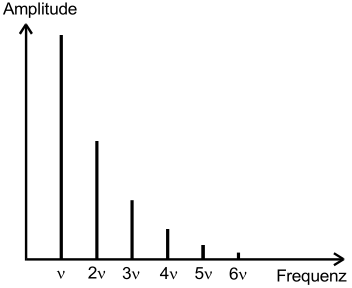
\includegraphics{Theorie1.png}
  \caption{Darstellung eines Linienspektrums einer periodischen Funktion [1].}
  \label{fig:1}
\end{figure}
